% Options for packages loaded elsewhere
\PassOptionsToPackage{unicode}{hyperref}
\PassOptionsToPackage{hyphens}{url}
\documentclass[
  9pt,
]{extarticle}
\usepackage{xcolor}
\usepackage[a5paper, margin=0.5cm]{geometry}
\usepackage{amsmath,amssymb}
\setcounter{secnumdepth}{-\maxdimen} % remove section numbering
\usepackage{iftex}
\ifPDFTeX
  \usepackage[T1]{fontenc}
  \usepackage[utf8]{inputenc}
  \usepackage{textcomp} % provide euro and other symbols
\else % if luatex or xetex
  \usepackage{unicode-math} % this also loads fontspec
  \defaultfontfeatures{Scale=MatchLowercase}
  \defaultfontfeatures[\rmfamily]{Ligatures=TeX,Scale=1}
\fi
\usepackage{lmodern}
\ifPDFTeX\else
  % xetex/luatex font selection
  \setmainfont[]{Latin Modern Roman}
\fi
% Use upquote if available, for straight quotes in verbatim environments
\IfFileExists{upquote.sty}{\usepackage{upquote}}{}
\IfFileExists{microtype.sty}{% use microtype if available
  \usepackage[]{microtype}
  \UseMicrotypeSet[protrusion]{basicmath} % disable protrusion for tt fonts
}{}
\makeatletter
\@ifundefined{KOMAClassName}{% if non-KOMA class
  \IfFileExists{parskip.sty}{%
    \usepackage{parskip}
  }{% else
    \setlength{\parindent}{0pt}
    \setlength{\parskip}{6pt plus 2pt minus 1pt}}
}{% if KOMA class
  \KOMAoptions{parskip=half}}
\makeatother
\usepackage{longtable,booktabs,array}
\usepackage{calc} % for calculating minipage widths
% Correct order of tables after \paragraph or \subparagraph
\usepackage{etoolbox}
\makeatletter
\patchcmd\longtable{\par}{\if@noskipsec\mbox{}\fi\par}{}{}
\makeatother
% Allow footnotes in longtable head/foot
\IfFileExists{footnotehyper.sty}{\usepackage{footnotehyper}}{\usepackage{footnote}}
\makesavenoteenv{longtable}
\usepackage{graphicx}
\makeatletter
\newsavebox\pandoc@box
\newcommand*\pandocbounded[1]{% scales image to fit in text height/width
  \sbox\pandoc@box{#1}%
  \Gscale@div\@tempa{\textheight}{\dimexpr\ht\pandoc@box+\dp\pandoc@box\relax}%
  \Gscale@div\@tempb{\linewidth}{\wd\pandoc@box}%
  \ifdim\@tempb\p@<\@tempa\p@\let\@tempa\@tempb\fi% select the smaller of both
  \ifdim\@tempa\p@<\p@\scalebox{\@tempa}{\usebox\pandoc@box}%
  \else\usebox{\pandoc@box}%
  \fi%
}
% Set default figure placement to htbp
\def\fps@figure{htbp}
\makeatother
\setlength{\emergencystretch}{3em} % prevent overfull lines
\providecommand{\tightlist}{%
  \setlength{\itemsep}{0pt}\setlength{\parskip}{0pt}}
\usepackage{multicol}
\usepackage{graphicx}
\usepackage{wrapfig}
\usepackage[svgnames]{xcolor}
\usepackage{float}
\usepackage{caption}
\usepackage{ifthen}
\usepackage{enumitem}
\setlist{nosep}
\linespread{1.2}
\setlength{\columnsep}{1cm}
\newboolean{inlatex}
\setboolean{inlatex}{true}
\usepackage{bookmark}
\IfFileExists{xurl.sty}{\usepackage{xurl}}{} % add URL line breaks if available
\urlstyle{same}
\hypersetup{
  pdftitle={KM271-WiFi Schnellstart-Anleitung},
  pdfauthor={Daniel (the78mole) Glaser},
  hidelinks,
  pdfcreator={LaTeX via pandoc}}

\title{KM271-WiFi Schnellstart-Anleitung}
\author{Daniel (the78mole) Glaser}
\date{\today}

\begin{document}
\maketitle

\section{KM271-WiFi Schnellstart}\label{km271-wifi-schnellstart}

Dies ist eine kurze Anleitung zur Inbetriebnahme des KM271-WiFi-Moduls.

  \begin{wrapfigure}{r}{0.40\textwidth}
    \centering
    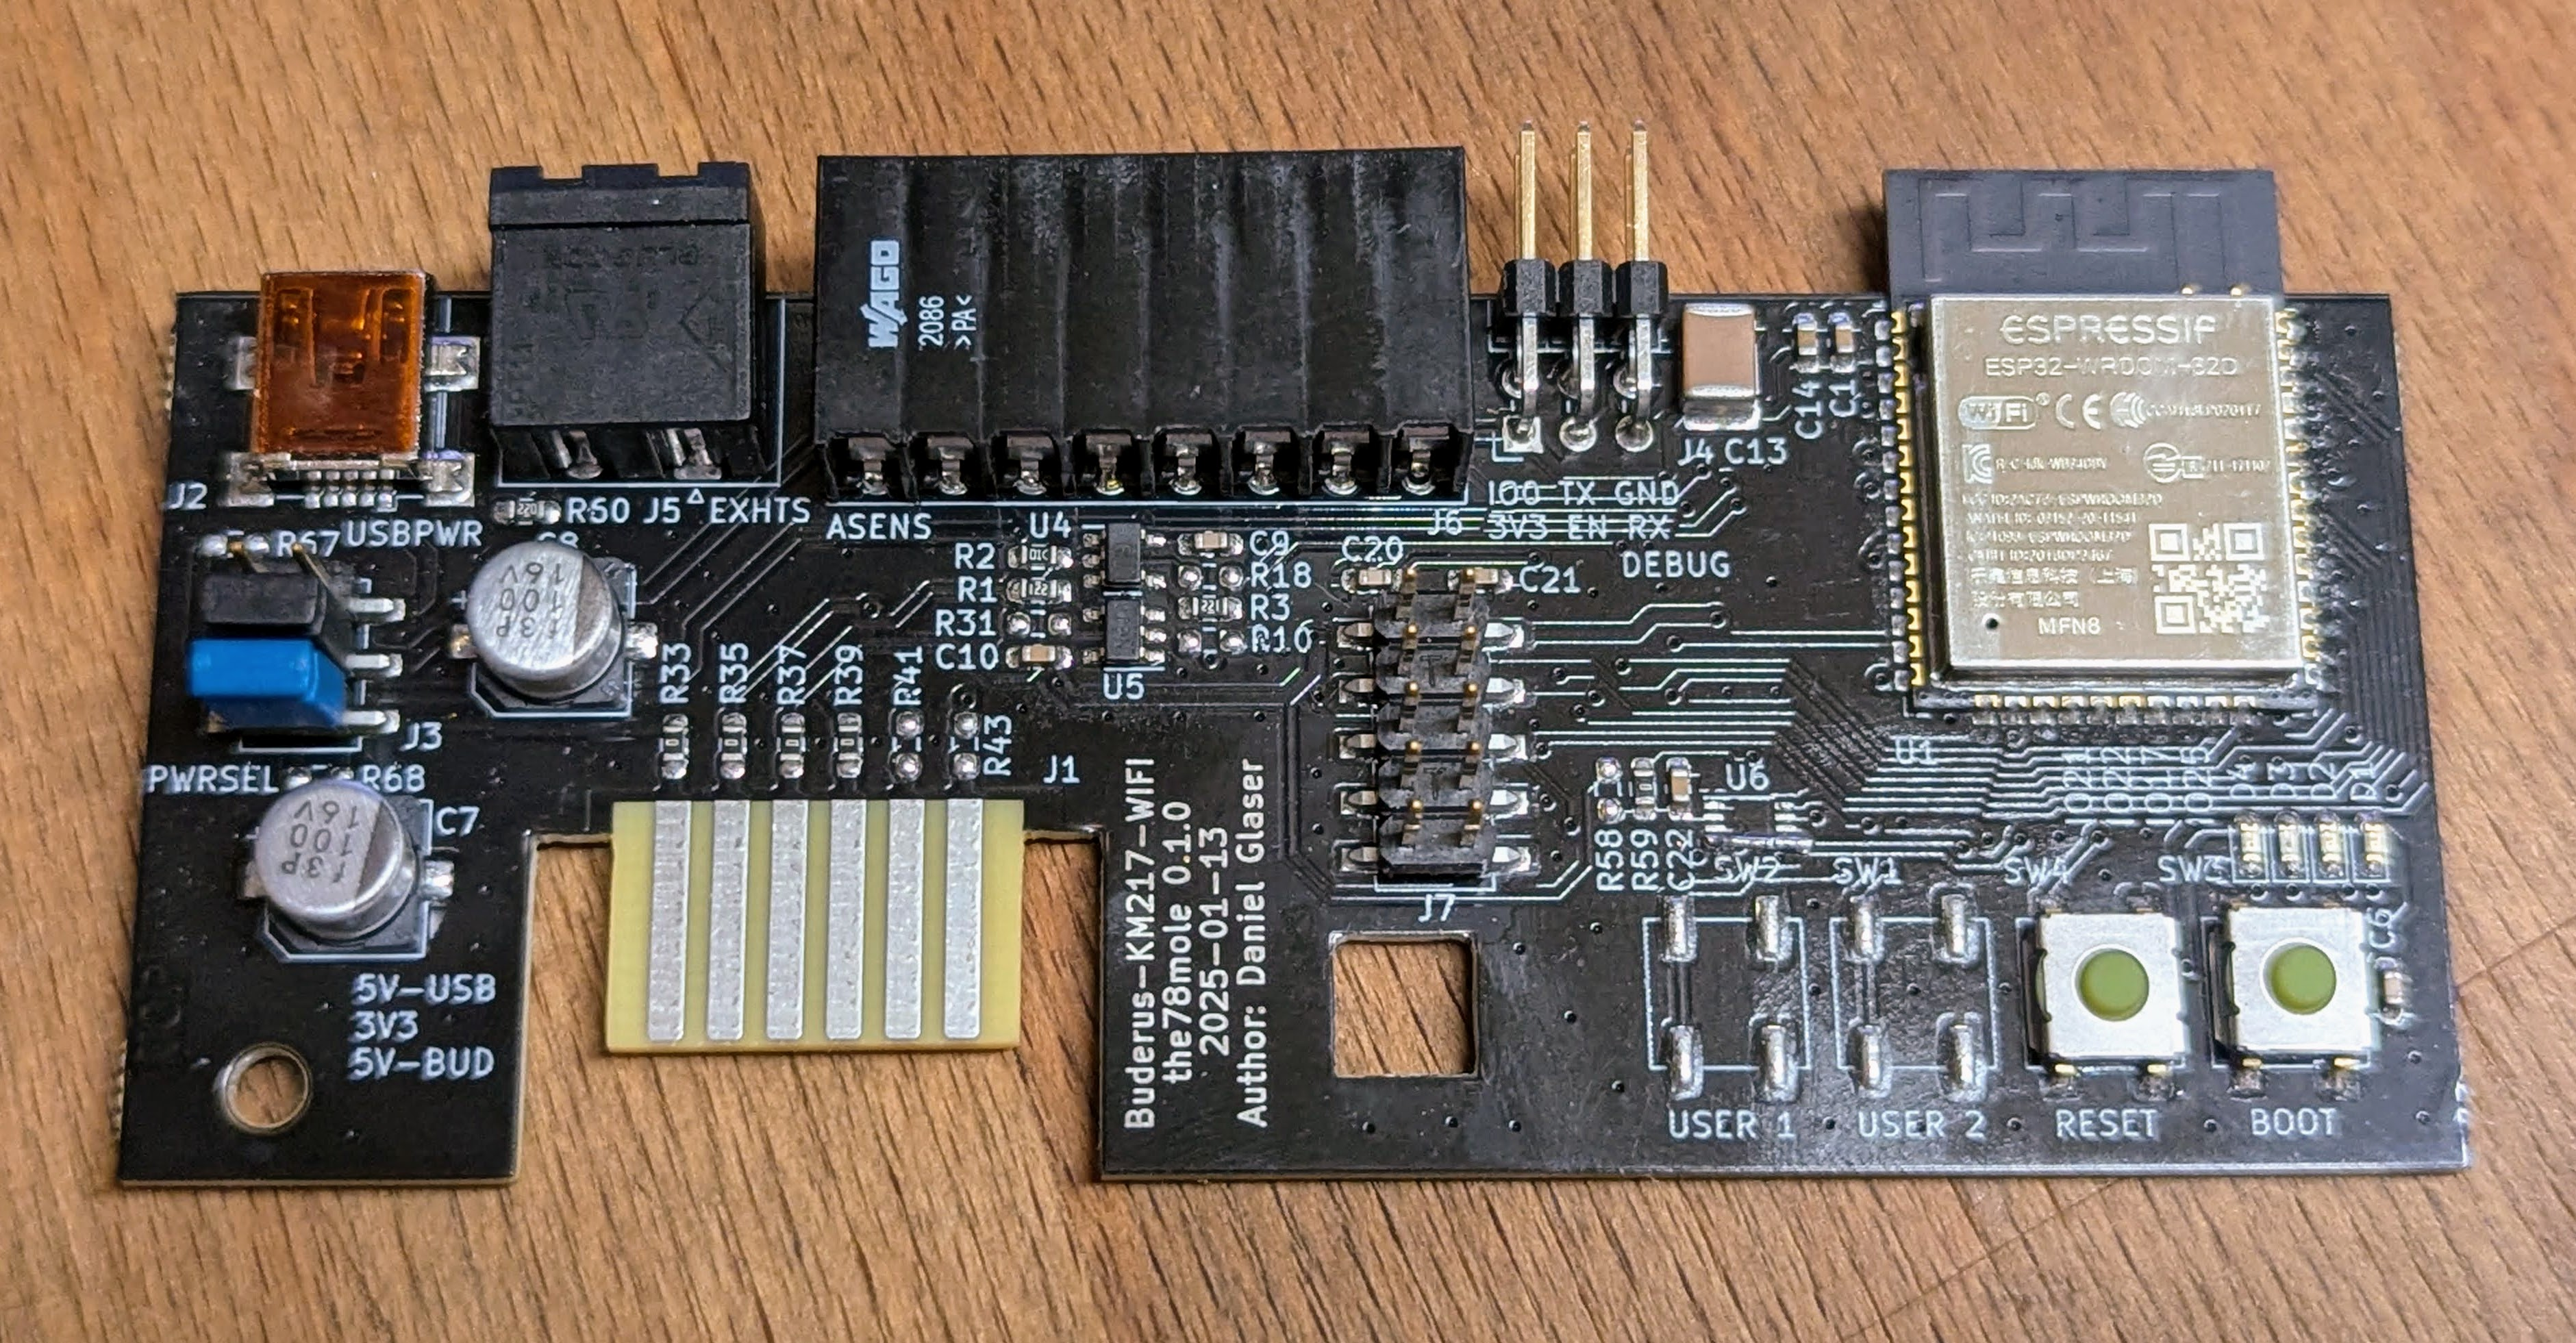
\includegraphics[width=0.38\textwidth]{../IMG/KM271-WiFi-0.1.0.jpg}
    \caption{KM271-WiFi groeßtenteils bestueckt}
  \end{wrapfigure}
  

\subsection{Voraussetzungen}\label{voraussetzungen}

Überprüfe zunächst, ob alles wie bestellt vorhanden ist (von links nach
rechts):

\begin{itemize}
\tightlist
\item
  \textbf{J5} ist der Anschluss für den Abgastemperatursensor (das
  Gegenstück lag dem Paket bei, Farben können abweichen: schwarz oder
  grün)
\item
  \textbf{J6} ist der Anschluss für Sensorleitungen
\item
  \textbf{J4} ist der Debug-Anschluss zur Programmierung über eine
  serielle Verbindung
\end{itemize}

Je nach Bestellung und gewählten Optionen sind einige Anschlüsse
möglicherweise nicht bestückt. Die Ethernet-Erweiterung auf dem zweiten
Bild ist ein separates Modul, das ebenfalls in meinem Tindie-Shop
erhältlich ist.

  \begin{wrapfigure}{r}{0.40\textwidth}
    \centering
    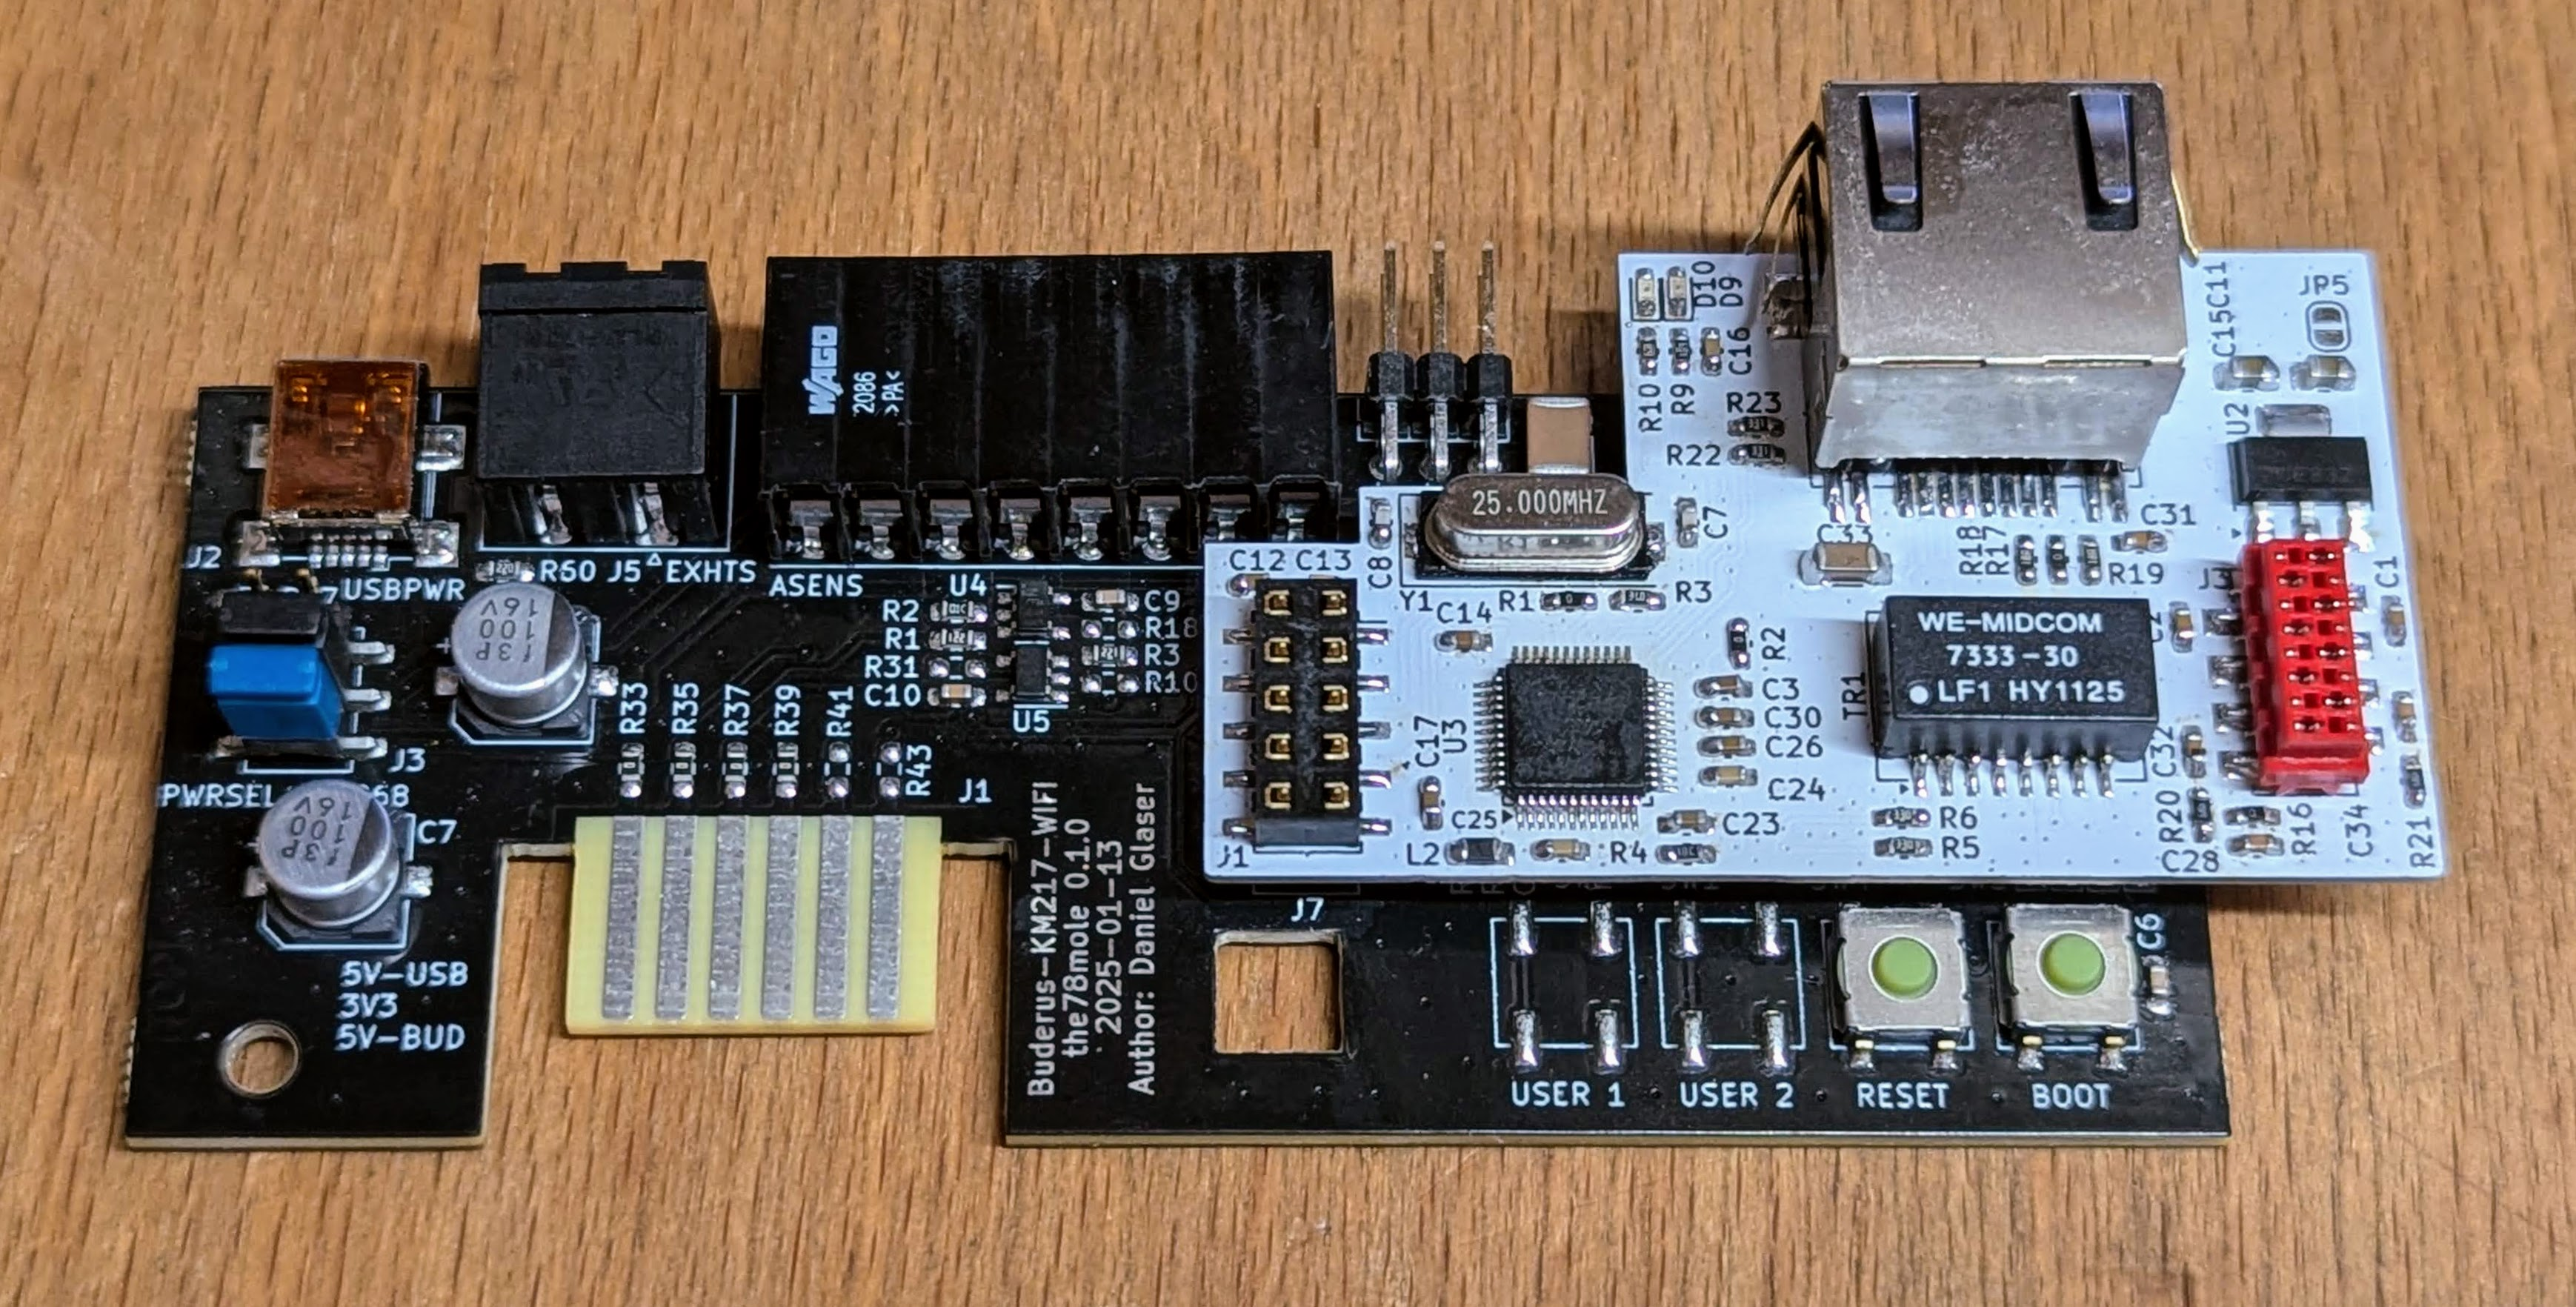
\includegraphics[width=0.38\textwidth]{../IMG/KM271-WiFi-0.1.0-ETH-Ext.jpg}
    \caption{KM271-WiFi mit Ethernet-Erweiterung}
  \end{wrapfigure}
  

Nun \textbf{prüfe, ob der PWRSEL-Header} wie im Bild gezeigt bestückt
ist. Der mittlere und der untere Jumper sollten gesteckt sein. Dies ist
die korrekte Variante für die \textbf{Versorgung über die
Buderus-Steuerung}. Wenn du das Modul \textbf{über USB versorgen}
willst, musst du den unteren Jumper (blau im Bild) nach oben versetzen.
Orientiere dich dabei an der Beschriftung unter dem Kondensator. Der
schwarze Jumper darf nur zum Flashen über die serielle Schnittstelle
entfernt werden.

Für die Ethernet-Erweiterung prüfe: J5 ist geschlossen, J4 ist offen,
und die Jumper J1 bis J3 sitzen auf den Positionen 2--3.

\subsection{Einbau}\label{einbau}

Wenn du Ethernet nutzen möchtest, ist jetzt der richtige Zeitpunkt, die
Ethernet-Erweiterung aufzustecken.

\begin{enumerate}
\def\labelenumi{\arabic{enumi}.}
\tightlist
\item
  Schalte die Buderus-Steuerung aus\\
\item
  Entferne die beiden Schrauben des Gehäuses und hebe es vorsichtig an\\
\item
  Biege die über dem KM271-Slot verlaufenden Kabel etwas nach oben,
  sodass das Modul seitlich eingeschoben werden kann\\
\item
  Richte das Modul in den Führungsschienen des KM271 aus und schiebe es
  nach unten\\
\item
  Drücke das Modul vorsichtig in den Steckplatz -- es rastet mit einer
  kleinen Lasche in die rechteckige Öffnung des KM271-Moduls ein (im
  Bild neben dem Flachsteckverbinder). Wenn du das Modul wieder
  entfernen möchtest, entriegle die Lasche mit einem Schraubendreher\\
\item
  Schließe ggf. weitere Sensoren an: Abgastemperaturfühler, Ölzähler,
  OneWire usw.\\
\item
  Setze das Gehäuse der Buderus-Steuerung wieder auf\\
\item
  Schalte die Steuerung wieder ein
\end{enumerate}

Auf dem Display der Buderus-Steuerung sollte nun ein neuer Eintrag
\texttt{ABGAS} oder \texttt{EXHAUST} erscheinen. Falls nicht, nutze das
Drehrad zur Navigation. Wenn du einen Abgastemperaturfühler
angeschlossen hast, wird dessen aktuelle Temperatur angezeigt. Falls
nicht, steht dort \texttt{-\/-\/-} -- das ist völlig in Ordnung.

Nun nimm dein Smartphone oder einen PC und suche nach dem WLAN
\texttt{Fallback\ Hotspot} (bei ESPhome) oder \texttt{ESP-Buderus-KM271}
(bei dewennis Firmware). Auf Android fragt das Gerät nach
10--20\,Sekunden, ob du verbunden bleiben möchtest (da keine
Internetverbindung vorhanden ist) -- bestätige mit \texttt{Ja}. Öffne
dann den Browser und rufe die Adresse http://192.168.4.1 auf. Manchmal
dauert es einige Minuten, bis eine Verbindung aufgebaut oder die Seite
geladen ist (vermutlich ein Bug in ESPhome). Bis zu diesem Punkt ist das
Vorgehen bei dewennis Firmware identisch -- sie reagiert meist nur etwas
schneller. Fahre jetzt mit dem passenden Kapitel zu deiner Firmware
fort.

\subsubsection{ESPhome-Konfiguration}\label{esphome-konfiguration}

Du solltest nun die Seite des Fallback-Hotspots sehen:

  \begin{wrapfigure}{r}{0.35\textwidth}
    \centering
    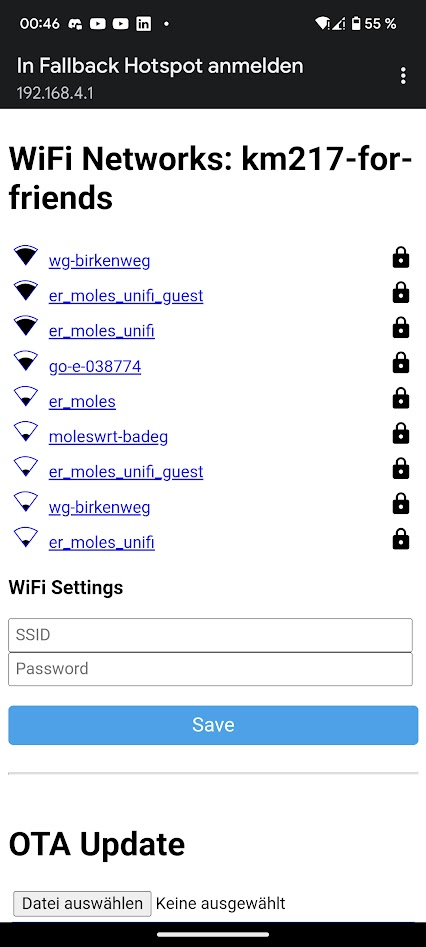
\includegraphics[width=0.33\textwidth]{../IMG/esphome-fallback-page.png}
    \caption{Fallback-Hotspot-Seite}
  \end{wrapfigure}
  

Wähle dein WLAN und gib das Passwort ein. Wenn du versehentlich das
falsche WLAN gewählt hast, ist es später schwierig, wieder Zugriff auf
das Board zu bekommen. In diesem Fall musst du das falsche WLAN
deaktivieren oder das Modul außerhalb der Reichweite bringen. Alternativ
kannst du das Modul aus der Buderus-Steuerung entfernen und per USB
versorgen und aus dem Empfangsbereich rausgehen (dazu den PWRSEL-Jumper
umsetzen). Danach kannst du die Einrichtung erneut starten.

Auf der Seite des Fallback-Hotspots kannst du auch eine neue Firmware
flashen -- allerdings \textbf{keine andere Firmware} (z.\,B. die von
dewenni).

Nach der Einrichtung sollte das Board in deinem ESPhome-Addon in Home
Assistant erscheinen. Du kannst nun die YAML-Konfiguration anpassen oder
so lassen, wie sie ist. Wenn eine neue Firmware verfügbar ist (z.\,B.
durch ein Update des Addons), kann diese in der Regel problemlos
eingespielt werden.

Das Gerät und seine Sensoren, Werte usw. findest du in Home Assistant
unter:\\
\textbf{Einstellungen → Geräte \& Dienste → ESPhome}

Weitere Informationen findest du hier:\\
https://github.com/the78mole/ESPhome-KM271-WiFi

\href{https://github.com/the78mole/ESPhome-KM271-WiFi}{\pandocbounded{\includegraphics[keepaspectratio]{https://api.qrserver.com/v1/create-qr-code/?data=https\%3A\%2F\%2Fgithub.com\%2Fthe78mole\%2FESPhome-KM271-WiFi&size=150x150}}}

\subsubsection{Dewennis
MQTT-Konfiguration}\label{dewennis-mqtt-konfiguration}

Beim ersten Zugriff auf dewennis Web-Oberfläche solltest du zunächst die
GPIOs konfigurieren -- insbesondere, wenn du die Ethernet-Erweiterung
(ETH-Ext) verwenden willst, um das KM271-WiFi mit deinem Heimnetz zu
verbinden. Die GPIOs sind wie folgt:

\begin{longtable}[]{@{}lll@{}}
\toprule\noalign{}
Signal & GPIO & Pin (J7) \\
\midrule\noalign{}
\endhead
\bottomrule\noalign{}
\endlastfoot
VCC & & J7.2 \\
GND & & J7.10 \\
CLK & 18 & J7.9 \\
MOSI & 23 & J7.7 \\
MISO & 19 & J7.5 \\
CS & 15 & J7.3 \\
INT & 14 & J7.8 \\
RST & 13 & J7.6 \\
\end{longtable}

Abgesehen von der Ethernet-Konfiguration kannst du alle weiteren
Einstellungen auch nach dem Neustart vornehmen.

Danach musst du noch die GPIOs für die Verbindung zur Buderus-Steuerung
konfigurieren. Für das KM271-WiFi gibt es eine vordefinierte Option --
bitte wähle diese aus. Wenn du andere Hardware anschließen möchtest,
findest du hier die detaillierte Beschreibung:

\href{https://bit.ly/4jA7aHu}{\pandocbounded{\includegraphics[keepaspectratio]{https://api.qrserver.com/v1/create-qr-code/?data=https\%3A\%2F\%2Fbit.ly\%2F4jA7aHu&size=150x150}}}

https://bit.ly/4jA7aHu

\begin{center}\rule{0.5\linewidth}{0.5pt}\end{center}

Für weitere Unterstützung kannst du meinem Matrix-Kanal beitreten:\\
https://matrix.to/\#/\%23molesblog:matrix.org

\begin{center}\rule{0.5\linewidth}{0.5pt}\end{center}

\textbf{Viel Spaß mit deinem Ölbrenner -- bis ihn die Wärmepumpe in
Rente schickt!}

\end{document}
